\documentclass[border=4pt]{standalone}
\usepackage{tikz}
\usetikzlibrary{arrows.meta,positioning,shapes.geometric}
\begin{document}
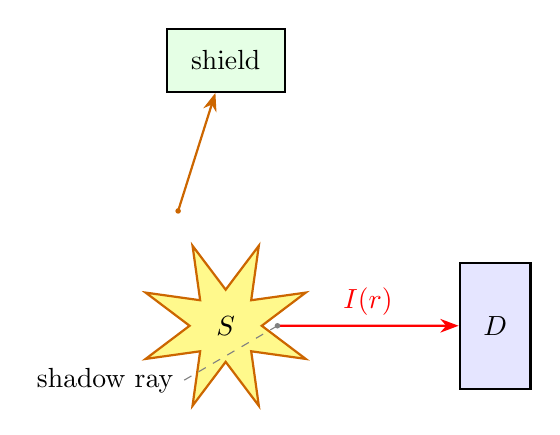
\begin{tikzpicture}[>=Stealth,node distance=23mm]
  \node[star,star points=8,star point ratio=2.4,star rotate=22.5,
    minimum size=22mm,outer sep=1.2mm,draw=orange!80!black,
    thick,fill=yellow!45] (source) {$S$};
  \node[draw,thick,right=of source,minimum width=9mm,minimum height=16mm,
    fill=blue!10] (detector) {$D$};
  \node[draw,thick,above=of source,minimum width=15mm,minimum height=8mm,
    fill=green!10] (shield) {shield};

  \draw[-Stealth,thick,red] (source) -- node[above] {$I(r)$} (detector);
  \draw[-Stealth,thick,orange!80!black] (source.outer point 1) -- (shield);
  \draw[dashed,gray] (source.inner point 6) -- ++(-12mm,-7mm)
    node[left,black] {shadow ray};
  \fill[orange!80!black] (source.outer point 1) circle (1pt);
  \fill[gray] (source.inner point 6) circle (1pt);
\end{tikzpicture}
\end{document}
